\documentclass{article}

\usepackage{graphicx}
\usepackage{listings}

\title{\vspace{-7em}Entity-Relationship Diagram}
\author{Isaac Boaz}

\begin{document}
\hspace*{-4cm}
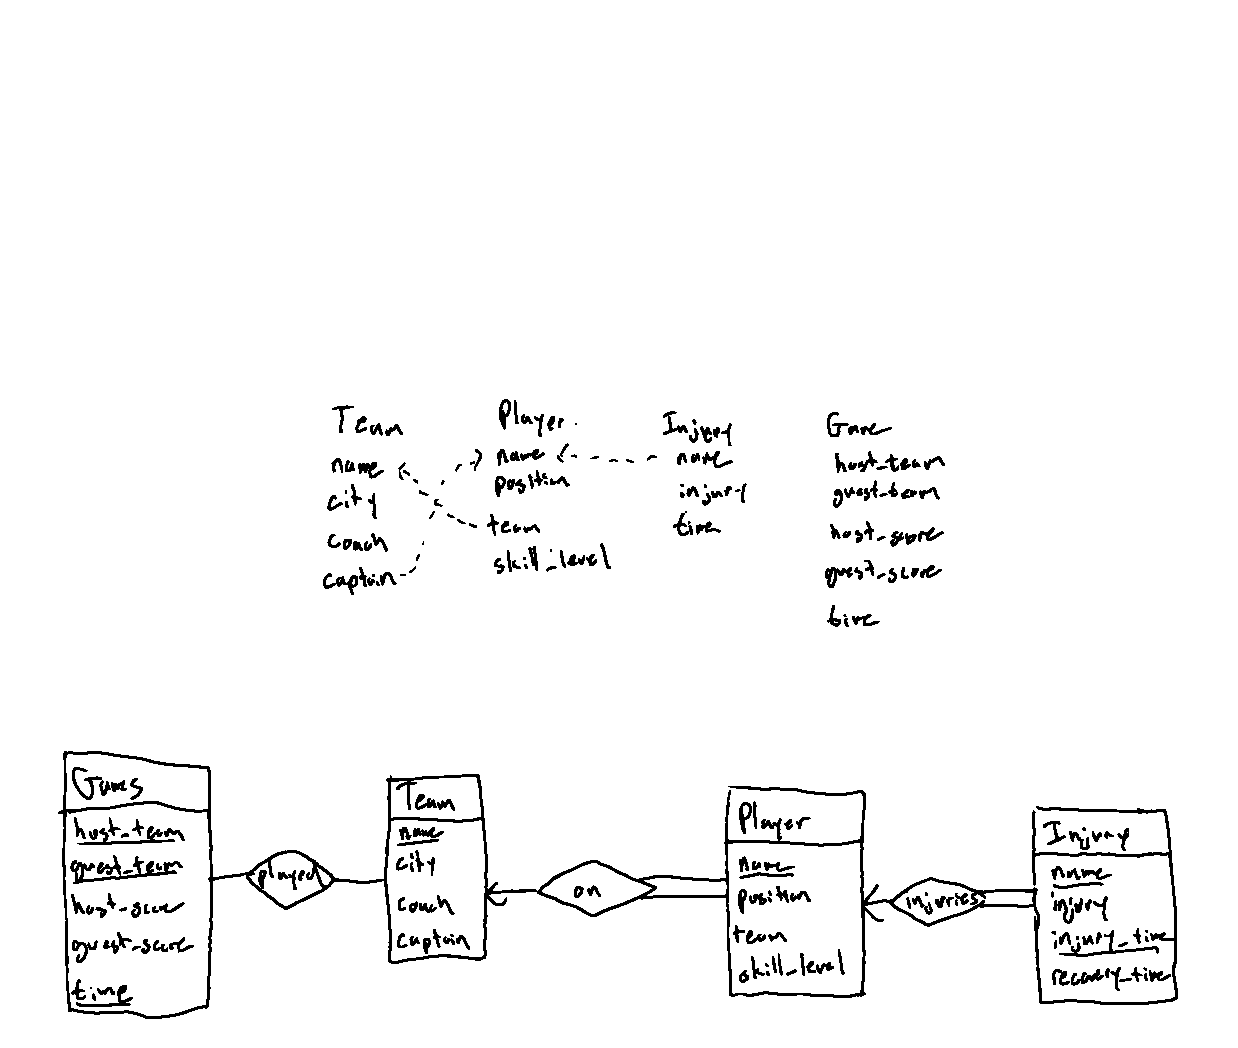
\includegraphics[page=1,angle=0,width=1.5\textwidth]{diagram.pdf}

\maketitle
\section*{Assumptions}
\begin{itemize}
    \item Player's skill is represented by a numeric value
    \item Player's names are guaranteed to be unique
    \item Injury records contain the date of the injury, the date of the player's return, and the injury type
\end{itemize}

\begin{lstlisting}[language=SQL]
CREATE TABLE Team (
    name VARCHAR(255) PRIMARY KEY,
    city VARCHAR(255),
    coach VARCHAR(255),
    captain VARCHAR(255),
    FOREIGN KEY (Captain) REFERENCES Player(name)
);

CREATE TABLE Player (
    name VARCHAR(255) PRIMARY KEY,
    position VARCHAR(255),
    skill_level INT,
    team VARCHAR(255),
    FOREIGN KEY (team) REFERENCES team(name)
);

CREATE TABLE Game (
    host_team VARCHAR(255),
    guest_team VARCHAR(255),
    time DATETIME,
    host_score INT,
    guest_score INT,
    PRIMARY KEY (host_team, guest_team, time),
    FOREIGN KEY (host_team) REFERENCES Team(name),
    FOREIGN KEY (guest_team) REFERENCES Team(name)
);

CREATE TABLE Injury (
    player VARCHAR(255),
    injury_date DATE,
    injury_type VARCHAR(255),
    recovery_time DATE,
    PRIMARY KEY (player, injury_date),
    FOREIGN KEY (player) REFERENCES Player(name)
);
\end{lstlisting}

\end{document}